% !TEX root = mythesis.tex

%==============================================================================
\chapter{The \tZqsec production}
\label{sec:tZq}
%==============================================================================

The proton-proton collisions occurring at high energies at the LHC allow 
multiple processes to occur. One of the
processes is the electroweak production of the \Ptop-quark and the 
\PZ-boson. The LO $t$-channel Feynman diagrams are shown in \cref{fig:tZqfeyn} where
a \PZ-boson can be radiated from any one of the incoming or outgoing quarks (\cref{fig:tZqfeyna})
or from the exchanged \PW-boson (\cref{fig:tZqfeynb}). In addition to these
resonant contributions, there is also a small non-resonant contribution 
in the form of $tl^+l^-q$ (\cref{fig:tZqfeync}) which is also accounted for. 
In this analysis, this process
is referred to as the \tZq production. 

\begin{figure}[htbp]
    \centering
    % \begin{subfigure}{0.35\figwidth}
    %   \centering
    %      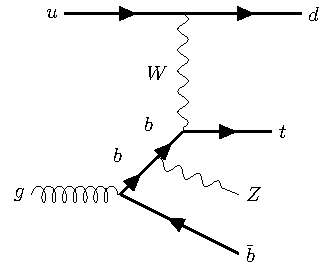
\includegraphics[width=\textwidth]{tZq_Zfromb.pdf}
    %      \caption{}
    %      \label{fig:tZqfeyna}
    % \end{subfigure}
    % \qquad
    \begin{subfigure}{0.35\figwidth}
      \centering
      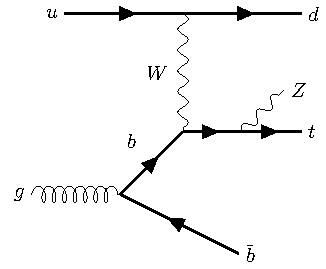
\includegraphics[width=\textwidth]{tZq_Zfromtop.pdf}
      \caption{}
      \label{fig:tZqfeyna}
    \end{subfigure}
    \begin{subfigure}{0.35\figwidth}
      \centering
      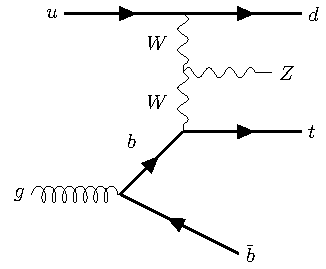
\includegraphics[width=\textwidth]{tZq_ZfromWW.pdf}
      \caption{}
      \label{fig:tZqfeynb}
    \end{subfigure}
  
  
  \medskip
  
  
  \begin{subfigure}{0.35\figwidth}
      \centering
      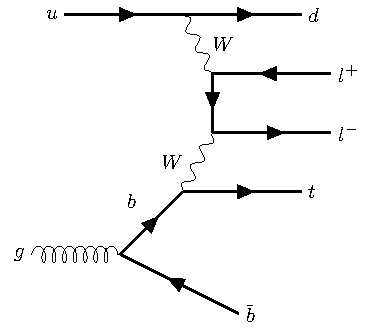
\includegraphics[width=\textwidth]{tZq_nonres.pdf}
      \caption{}
         \label{fig:tZqfeync}
    \end{subfigure}
    % \begin{subfigure}{0.35\figwidth}
    %   \centering
    %   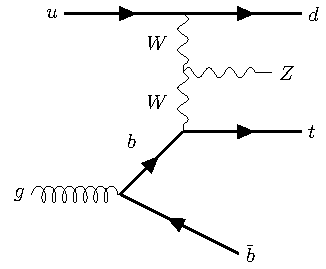
\includegraphics[width=\textwidth]{tZq_ZfromWW.pdf}
    %   \caption{}
    %      \label{fig:tZqfeyne}
    % \end{subfigure}
    % \begin{subfigure}{0.35\figwidth}
    %     \centering
    %     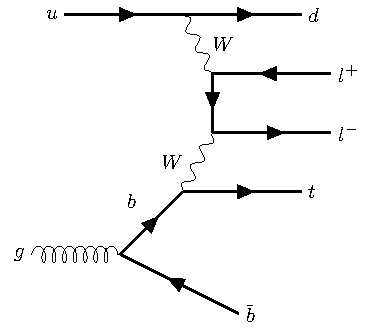
\includegraphics[width=\textwidth]{tZq_nonres.pdf}
    %     \caption{}
    %      \label{fig:tZqfeynf}
    %   \end{subfigure}
  
  \caption[Feynman diagrams at LO for the \tZq-production]{Feynman diagrams at 
  LO for the \tZq-production. The \PZ is radiated either from one of the
  quarks or from the exchanged W boson. }
  \label{fig:tZqfeyn}
  \end{figure}

The \tZq production is interesting to study because it probes the coupling
of a fermion to a fermion and a fermion to a boson in the same interaction. Moreover, 
it can provide a solid basis to study $tHq$ process. It is important to note 
that the particles involved in this production are quite heavy and therefore,
the only way to spot them is from their reconstructed decay products. 
Conventionally, the final states are divided into several \textit{channels}
based on certain combination of leptons and jets. This analysis focuses on
the so-called trilepton channel.

\section{The \tZqsec Trilepton Channel}
As the name suggests, the trilepton decay channel of the \tZq production 
contains final states with three charged leptons, the probability of which
is very small. However, the charged leptons allow for a clean signature
of this final state and therefore, \tZq is studied in the trilepton channel. This
is referred to as our signal.

\begin{figure}
  \centering
      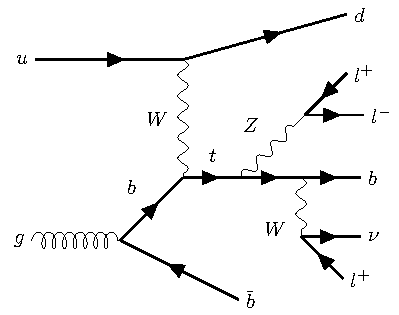
\includegraphics[width=0.5\textwidth]{tZq_Zfromtop_decay.pdf}
      \caption{The \tZq trilepton final state}
         \label{fig:tZqtrilep}
\end{figure}

In order to reconstruct the trilepton final state, as shown in \cref{fig:tZqtrilep}, certain 
requirements are imposed on the recorded detector data, specifically on leptons, jets and
\mynote{missing transverse energy}{What cut?}. The collection of these requirements is called the event selection
which in this scenario, is geared to selecting events containing \tZq trilepton 
signatures. It is summarised in \cref{tab:selection:srcr}.

Primary requirements are as follows:

\begin{itemize}
  \item \textbf{Leptons}
    \begin{itemize}
      \item Exactly three leptons (\Pelectron or \Pmu)
      \footnote{\Ptau is considered if it decays into leptons}. These leptons are 
      sorted by their \pT which is required to be at least 27,15 and 10 GeV, respectively.
      
      \item At least 1 Opposite Sign Same Flavour (OSSF) lepton pair with a minimum
      difference between its invariant mass ($m_{ll}$) and $m_Z$. This is to identify 
      which out of the selected leptons originate from \PZ.

      \item A cut on minimum accepted invariant mass, in order to suppress backgrounds 
      not containing a \PZ.

      \item \mynote{mTw, MET?}{Reason?}
  \end{itemize}
  \item \textbf{Jets}
  \begin{itemize}
    \item Number of jets are required to be between 2 and 5, with \pT more than \qty{25}{GeV}
    and $|\eta|$ more than 4.5.
    \item Number of \Pbottom-jets are required to be 1 or 2, reconstructed at $85\%$ working 
    point with $|\eta|$ more than 2.5. Events with 2 jets, both \Pbottom-tagged are nor considered.
  \end{itemize}


\end{itemize}

\begin{table}[!htbp]
    \footnotesize
    \caption{Event selection}
    \label{tab:selection:srcr}
    \renewcommand{\arraystretch}{1.3}
    \centering
    \begin{tabular}{lccc}
        \toprule
        Variable & \multicolumn{3}{c}{Preselection}\\
        \midrule
        $N_\ell~\left(\ell=e,\mu\right)$ & \multicolumn{3}{c}{$=3$}\\
        & \multicolumn{3}{c}{$\ge 1$ OSSF lepton pair}\\
        $\pT\left(\ell_1,\ell_2,\ell_3\right)$ & \multicolumn{3}{c}{$>$ 27,~15, \qty{10}{\GeV}}\\
        $\min(m_{\ell\ell})$ & \multicolumn{3}{c}{$>$ \qty{20}{\GeV}} \\
        $|m_{\ell\ell} - m_{Z}|$ & \multicolumn{3}{c}{$<$ \qty{10}{\GeV}} \\
        \mtw & \multicolumn{3}{c}{$>$ \qty{30}{\GeV}} \\
        $N_\text{jets}\left(\pT>25~\mathrm{GeV}\right)$ & \multicolumn{3}{c}{2-5} \\
        $N_{b-\text{jets}} @ 85\%$ & \multicolumn{3}{c}{1-2 (no $2j2b$)} \\
        % & SR & \CRttZ & \CRVV \\
        % $N_\text{jets}\left(\pT>25~\mathrm{GeV}\right)$ & 2-5 & $\ge 6$ & 2-5 \\
        % $N_{b-\text{jets}} @ 85\%$ & 1-2 (no $2j2b$) & $\ge 1$ & 0 \\
        \bottomrule
    \end{tabular}
    \end{table}


It is important to note here that these requirements are chosen to 
maximise the probability of selecting signal events
but in reality there are background processes that mimic the \tZq signature
and therefore, contaminate the selected signal events. 

\section{Background processes}
